\section{Datasets}
\label{sec:datasets}

Several benchmarks study spatial reasoning, including SpatialRGPT-Bench~\cite{spatialRGPT} and $3$DSRBench~\cite{3dsrbench}, but their primary modality is single-image VQA, which precludes evaluation of (i) viewpoint consistency, (ii) partial observability, and (iii) the need for exploration before committing to an answer. Embodied QA benchmarks such as HM-EQA~\cite{ren2024exploreconfidentefficientexploration}, used as an evaluation set by systems like GraphEQA~\cite{graphEQA}, %\opnote{HM-EQA is not from graph-EQA?? also GraphEQA is not a benchmark?}
move closer by emphasizing interaction and persistent memory, but target semantic or factual questions rather than \emph{metric--semantic--predicate} grounding (e.g., ``$2\,\mathrm{m}$ left of the chair'') as an evaluation target.

To isolate $3$D metric goal grounding, we introduce \textbf{MAPG-Bench} (Map-based Anchored Predicate Grounding Benchmark). MAPG-Bench contains $98$ human-annotated queries across $41$ HM$3$D~\cite{ramakrishnan2021habitatmatterport3ddatasethm3d} indoor scenes rendered in Habitat-Sim. %\opnote{How many queries in total??? Are all metric or are some object based too?}
It comprises two complementary query types: \textbf{Object-to-World (O-W)} queries require localizing a continuous $3$D allocentric waypoint relative to an anchor object (e.g., ``Where is $2\,\mathrm{m}$ to the right of the fridge?''), and \textbf{Object-to-Object (O-O)} queries require selecting the correct instance among multiple candidates satisfying a relational predicate (e.g., ``Which chair is in front of the sofa?''). 
% \opnote{If you have both- you need to introduce O-O and O-W here and specify how many of both are present in the dataset. If not you're good. This is important cause you liberally use O-O and O-W without introducing them formally as a part of your benchmark. You also need to say where those terms come from (cite the paper).}

Annotations were collected with an interactive tool that overlays semantic instance labels on the agent's egocentric view. Annotators explored each scene, selected anchor instances, and recorded the agent's pose. For O-W queries, the ground truth is an explicit $3$D allocentric point placed on a navigable surface, an actionable waypoint rather than a text description. Predicates cover three families: horizontal directional (\texttt{in-front-of} $33$, \texttt{right-of} $18$, \texttt{behind} $13$, \texttt{left-of} $11$), vertical (\texttt{above} $10$, \texttt{below} $4$), and relational (\texttt{between} $6$, \texttt{near} $1$, \texttt{towards} $1$, \texttt{from} $1$). Metric distances span typical indoor scales ($0.5$--$4.0\,\mathrm{m}$); a further $6$ queries carry no metric offset ($d_0=0$) and serve as purely directional controls. A specialized \emph{commonsense} subset probes VLM failures on intrinsic frame-of-reference predicates, where the ``front'' of an object is defined by its affordance direction rather than the camera's line of sight, a systematically hard case documented in~\cite{frameOfReferenceAmbiguity}.

\begin{figure}[!t]
  \centering
  \vspace{2mm}
  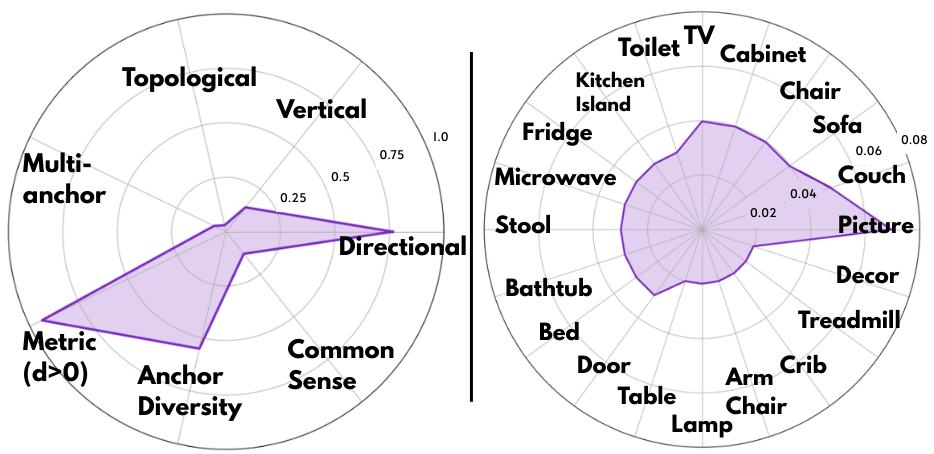
\includegraphics[width=0.90\linewidth,height=10cm,keepaspectratio]{figures/fig_5.png}
  \caption{\textbf{Distribution} of query categories (left) and anchor object labels (right) in MAPG-Bench. \rev{Example queries: (O-W, metric) ``Where is $2\,\mathrm{m}$ to the right of the fridge?''; (O-W, directional) ``Where is directly behind the sofa?''; (O-O) ``Which chair is nearest to the window?''; (commonsense) ``Where is in front of the armchair?'' (resolved via affordance direction).} %\opnote{IMP: You should extend this figure and how 3-4 examples of the queries you have added in mapg-bench. This can go in the caption too.}
  }
  \label{fig:mapg_distributions}
\end{figure}